\section{検証目的}
IoT機器の監視・管理の際の問題が解決できたのか,検証を行う.
\begin{itemize}
\item IoT機器が多量であるため,監視サーバへの登録も負担となる.
\item IoT機器が接続されるネットワークが多様であるため,既存の問い合わせによる監視手法は適応できない.
\item IoT機器の追加や交換が頻繁にあるため,監視サーバへの登録作業を頻繁に行う必要がある.
\item 外観が似通っているため,交換のため現地に行くも,交換すべき機器がどれなのか判別がつかない.
\end{itemize}
これら問題から、監視サーバへの登録の負担が軽減されている事と、機器からの通知による監視が行えているのか検証を行った。

\begin{comment}
実装の都合から,この3つの要件の中で機器からの通知に基づいた監視のみの検証を行う.
機器から,機器IDと接続出来なかった回数等を,デバイスIDに紐付いたURLに送信し,監視サービスにて,監視することができることを確認する.
そのため,各IoT機器に対する設定・サーバでの登録は,手動で行う.
\end{comment}

\section{検証方法}
検証は次のような小規模なIoTサービスを想定し,行った.
IoT機器の数は,1台とし,RaspberryPi2を使用することとした.
OSはRaspbeian jessieがインストールされていることとした.
図\ref{fig:device}は使用したRaspberryPi2と,IntelEdisonである.
今回は,IntelEdisonは使用していないが,参考の為に上げた.
%IoT機器の図
\begin{figure}[htbp]
\begin{center}
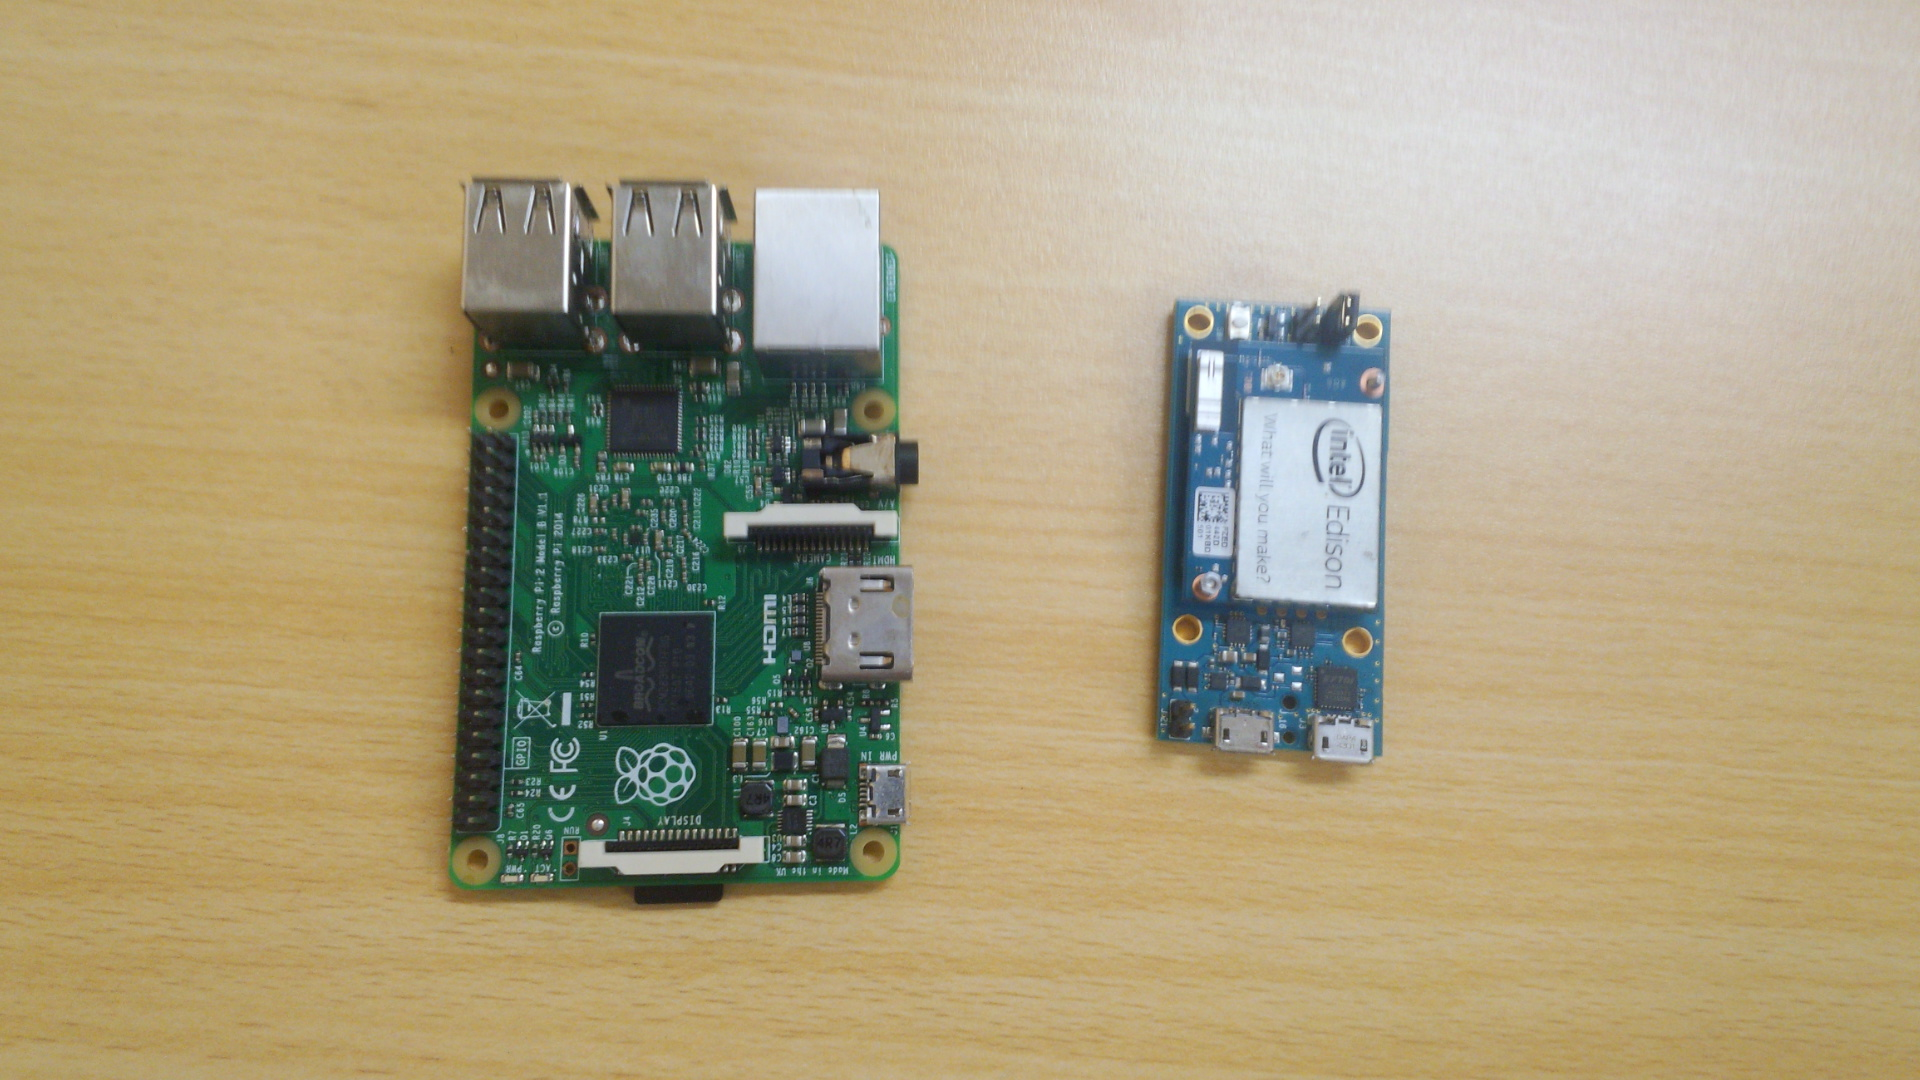
\includegraphics[width=14cm]{images/device.png}
\caption{RaspberryPi2とIntelEdison}
\label{fig:device}
\end{center}
\end{figure}

RaspberyPi2は無線LANインターフェースを持たないので,バファロー製の無線LANインターフェースを使用した.
期間は2017年1月28日正午から1時間行い,途中何度かIoT機器の電源を抜き,正常に検知することを確認する.
また,期間初めに,想定するIoT機器の設定を行い,監視サービスにて発行したIDを設定する.

\section{検証結果}
本サービスを利用した監視について、作業別に確認した。
\begin{enumerate}

\item 登録・設定\\
まず,サービス側で機器IDの登録を行った.
ブラウザからサービスへログインし,登録ボタンをクリックして,登録用ダイアログを開いた.
図\ref{fig:ss_regist}は登録用ダイアログのスクリーンショットである。

ここで,登録用ダイアログに表示されているIDをコピーしておく.
登録用ダイアログにて,機器名と機器の詳細(機器名を「RaspberryPi A」,機器の詳細を「TestDeviceA」とした)を入力し,登録ボタンを押した.
その後,サービスの画面上に「RaspberryPi A」という名前を持つデバイスが作成されたことを確認した.
図\ref{fig:ss_main}は監視サービスメイン画面のスクリーンショットである.
\medskip

次に,エージェントプログラムを機器のSDカードのホームディレクトリとなるディレクトリ(/home/pi/)へ,agent.shという名前で書き込んだ.
また,起動時にエージェントプログラムを実行するための設定ファイルを機器のSDカードの設定用ディレクトリ(/etc/sysytemd/system/)へ,devmon.serviceという名前で書き込んだ.
この設定ファイルは,起動時に/home/pi/agent.shのスクリプトを機器IDを引数として実行するように指定している.
\medskip

従来の機器からの通知による監視手法では、
登録の際に、監視サーバ上にある設定ファイルを開き、機器固有のホスト名や通知の送信先等を入力し、IoT機器側でも設定ファイルを開き、サーバ上の設定ファイルの内容と相違無く編集する必要があった。
本手法では、機器への設定はIDだけとなり、監視サーバの設定ファイルを開く必要がなくなった。
また、各設定の整合性は、サーバがIDを管理することで行うことができているため、考慮する必要がなくなった。
このことから、監視サーバと機器への設定が省力化された事が確認できる。

\item 運用\\
その後,機器の電源を入れ,機器上でエージェントプログラムが稼働していることを,systemctl statusコマンドを用いて確認した.
また,サービス側で指定したIDを持つ機器の状態が異常状態(稼働していないかネットワークから切断されている事を表す)から,
正常状態(稼働していて,ネットワークが切断されていない事を表す)へ変化した事を確認した.
機器から該当のIDに紐付いたURLに対し,通信が出来ている場合のみ,正常状態となるので,正常にIDとURLが紐付いている事が確認できたといえる.

このことから、機器からの通知による監視が行えていることを確認できた。
\item トラブルの検知・機器の移動\\
電源ケーブルを抜き,サービス上で該当の機器の状態が正常状態から異常状態へ変化することを確認した.
変化には2分程度かかり,これは,機器が1分おきに通知を行っていることと,ブラウザ側のプログラムにて1分おきにサーバへ該当機器の状態を問い合わせているためである.
再度電源ケーブルを挿し直すと,1分程度でサービス上の機器の表示が異常状態から正常状態へ変化した.
また、機器上にて機器のIPアドレスを変更し、異常として検知されないことを確認した。

このことから、機器からの通知による監視が行えていること、移動などの場合であっても、監視サーバやIoT機器の設定を変更しなくて良い事を確認した。
\end{enumerate}
これらから、監視サーバへの登録の負担が軽減され、機器からの通知による監視が行えている事が分かった。







\begin{comment}
\begin{enumerate}
\item 予め固有のIDとエージェントプログラムがインストールされた機器を買ってくる
\item ユーザは,その機器に対しサービスで利用するアプリケーションをインストールし,設置する
\item 機器は,設置後ネットワークに接続され次第,サービスへ,機器の状態の通知を行う
\end{enumerate}
IoTサービス提供者が手軽に利用できることを確認した.

\section{サービスの特徴}
他の関し手法と比較した本サービスの特徴として,通知型で設定不要,規模に対応できることが挙げられる.
独立したサービスとしてまとまっていることが挙げられる.
\end{comment}

\section{考察}
提案する方法でIoT機器からの監視が行えることは分かったが,下記問題については実装の都合上,確認が取れていない.
\begin{itemize}
\item 各IoT機器の状態を監視するために,多数のIoT機器へ設定をしなければいけない負担
\item 増減や交換の度に,機器監視システムへの登録をしなければならない負担
\end{itemize}
今後,実装を進め,検証を行うこととする.

また,検証に置いて次のような改善点が見つかった.
\begin{itemize}
\item 過去の記録の表示\\
	現在,過去の機器状態の記録については,文字記録として表示しているが,グラフ表示等の方が見やすいと感じた.
	また,期間を指定して閲覧できる機能も必要であることが分かった.
\item アラート機能\\
	監視サービスの画面を見続けるわけには行かないので,メール等によるアラート機能等を追加する必要があると感じた
\item グループ表示機能\\
	グループ表示等が行えると尚見やすい事が分かった.
\item 一覧表示\\
	機器が少量である場合は問題ないが,数千台となった場合に,一覧での表示は,見難い事が分かった.
	全体やグループでの稼働率等を表示し,確認が必要な機器のみを一覧で表示する等の工夫が必要となることがわかった.
\end{itemize}
また,本来ならば,IoTサービスを提供している企業に使用して頂き,評価を得る必要があったが,双方のスケジュールの都合と開発の遅れから行うことが出来なかった.
しかし,今後IoTサービスの開発が盛んになることや,使用するIoT機器の数が多くなることから,本サービスの必要性は高くなっていくと考えられる.

